\documentclass[a4paper,justified,final,twoside,nobib]{tufte-book}

\hypersetup{colorlinks}% uncomment this line if you prefer colored hyperlinks (e.g., for onscreen viewing)

\usepackage{mathtools} %added mathtools for piecewise functions

%%
% Book metadata
\title{A\\Machine Learning\\Handbook\thanks{Thanks to Edward R.~Tufte for his inspiration.}}
\author[]{}
\publisher{Publisher of This Book}

%%
% Automated bibliography management
\usepackage{natbib}
\setcitestyle{authoryear}

%%
% If they're installed, use Bergamo and Chantilly from www.fontsite.com.
% They're clones of Bembo and Gill Sans, respectively.
%\IfFileExists{bergamo.sty}{\usepackage[osf]{bergamo}}{}% Bembo
%\IfFileExists{chantill.sty}{\usepackage{chantill}}{}% Gill Sans

\usepackage{microtype}

%%
% Describe algorithms using fancy pseudo code
\usepackage{algorithm}
\usepackage[noend]{algpseudocode}

%%
% Just some sample text
\usepackage{lipsum}
\usepackage{soul}
%%
% For nicely typeset tabular material
\usepackage{booktabs}
\usepackage{pdfpages}

%%
% For graphics / images
\usepackage{graphicx}
\setkeys{Gin}{width=\linewidth,totalheight=\textheight,keepaspectratio}
\graphicspath{{graphics/}}

% The fancyvrb package lets us customize the formatting of verbatim
% environments.  We use a slightly smaller font.
\usepackage{fancyvrb}
\fvset{fontsize=\normalsize}

%%
% Prints argument within hanging parentheses (i.e., parentheses that take
% up no horizontal space).  Useful in tabular environments.
\newcommand{\hangp}[1]{\makebox[0pt][r]{(}#1\makebox[0pt][l]{)}}

%%
% Prints an asterisk that takes up no horizontal space.
% Useful in tabular environments.
\newcommand{\hangstar}{\makebox[0pt][l]{*}}

%%
% Prints a trailing space in a smart way.
\usepackage{xspace}

%%
% Some shortcuts for Tufte's book titles.  The lowercase commands will
% produce the initials of the book title in italics.  The all-caps commands
% will print out the full title of the book in italics.
\newcommand{\vdqi}{\textit{VDQI}\xspace}
\newcommand{\ei}{\textit{EI}\xspace}
\newcommand{\ve}{\textit{VE}\xspace}
\newcommand{\be}{\textit{BE}\xspace}
\newcommand{\VDQI}{\textit{The Visual Display of Quantitative Information}\xspace}
\newcommand{\EI}{\textit{Envisioning Information}\xspace}
\newcommand{\VE}{\textit{Visual Explanations}\xspace}
\newcommand{\BE}{\textit{Beautiful Evidence}\xspace}
\newcommand{\ics}{\smallcaps{ICS5110 Applied Machine Learning\xspace}}

\newcommand{\TL}{Tufte-\LaTeX\xspace}

% Prints the month name (e.g., January) and the year (e.g., 2008)
\newcommand{\monthyear}{%
  \ifcase\month\or January\or February\or March\or April\or May\or June\or
  July\or August\or September\or October\or November\or
  December\fi\space\number\year
}

% Prints an epigraph and speaker in sans serif, all-caps type.
\newcommand{\openepigraph}[2]{%
  %\sffamily\fontsize{14}{16}\selectfont
  \begin{fullwidth}
  \sffamily\large
  \begin{doublespace}
  \noindent\allcaps{#1}\\% epigraph
  \noindent\allcaps{#2}% author
  \end{doublespace}
  \end{fullwidth}
}

% Inserts a blank page
\newcommand{\blankpage}{\newpage\hbox{}\thispagestyle{empty}\newpage}

\usepackage{units}

% Typesets the font size, leading, and measure in the form of 10/12x26 pc.
\newcommand{\measure}[3]{#1/#2$\times$\unit[#3]{pc}}

% Macros for typesetting the documentation
\newcommand{\hlred}[1]{\textcolor{Maroon}{#1}}% prints in red
\newcommand{\hangleft}[1]{\makebox[0pt][r]{#1}}
\newcommand{\hairsp}{\hspace{1pt}}% hair space
\newcommand{\hquad}{\hskip0.5em\relax}% half quad space
\newcommand{\TODO}{\textcolor{red}{\bf TODO!}\xspace}
\newcommand{\ie}{\textit{i.\hairsp{}e.}\xspace}
\newcommand{\eg}{\textit{e.\hairsp{}g.}\xspace}
\newcommand{\na}{\quad--}% used in tables for N/A cells
\providecommand{\XeLaTeX}{X\lower.5ex\hbox{\kern-0.15em\reflectbox{E}}\kern-0.1em\LaTeX}
\newcommand{\tXeLaTeX}{\XeLaTeX\index{XeLaTeX@\protect\XeLaTeX}}
% \index{\texttt{\textbackslash xyz}@\hangleft{\texttt{\textbackslash}}\texttt{xyz}}
\newcommand{\tuftebs}{\symbol{'134}}% a backslash in tt type in OT1/T1
\newcommand{\doccmdnoindex}[2][]{\texttt{\tuftebs#2}}% command name -- adds backslash automatically (and doesn't add cmd to the index)
\newcommand{\doccmddef}[2][]{%
  \hlred{\texttt{\tuftebs#2}}\label{cmd:#2}%
  \ifthenelse{\isempty{#1}}%
    {% add the command to the index
      \index{#2 command@\protect\hangleft{\texttt{\tuftebs}}\texttt{#2}}% command name
    }%
    {% add the command and package to the index
      \index{#2 command@\protect\hangleft{\texttt{\tuftebs}}\texttt{#2} (\texttt{#1} package)}% command name
      \index{#1 package@\texttt{#1} package}\index{packages!#1@\texttt{#1}}% package name
    }%
}% command name -- adds backslash automatically
\newcommand{\doccmd}[2][]{%
  \texttt{\tuftebs#2}%
  \ifthenelse{\isempty{#1}}%
    {% add the command to the index
      \index{#2 command@\protect\hangleft{\texttt{\tuftebs}}\texttt{#2}}% command name
    }%
    {% add the command and package to the index
      \index{#2 command@\protect\hangleft{\texttt{\tuftebs}}\texttt{#2} (\texttt{#1} package)}% command name
      \index{#1 package@\texttt{#1} package}\index{packages!#1@\texttt{#1}}% package name
    }%
}% command name -- adds backslash automatically
\newcommand{\docopt}[1]{\ensuremath{\langle}\textrm{\textit{#1}}\ensuremath{\rangle}}% optional command argument
\newcommand{\docarg}[1]{\textrm{\textit{#1}}}% (required) command argument
\newenvironment{docspec}{\begin{quotation}\ttfamily\parskip0pt\parindent0pt\ignorespaces}{\end{quotation}}% command specification environment
\newcommand{\docenv}[1]{\texttt{#1}\index{#1 environment@\texttt{#1} environment}\index{environments!#1@\texttt{#1}}}% environment name
\newcommand{\docenvdef}[1]{\hlred{\texttt{#1}}\label{env:#1}\index{#1 environment@\texttt{#1} environment}\index{environments!#1@\texttt{#1}}}% environment name
\newcommand{\docpkg}[1]{\texttt{#1}\index{#1 package@\texttt{#1} package}\index{packages!#1@\texttt{#1}}}% package name
\newcommand{\doccls}[1]{\texttt{#1}}% document class name
\newcommand{\docclsopt}[1]{\texttt{#1}\index{#1 class option@\texttt{#1} class option}\index{class options!#1@\texttt{#1}}}% document class option name
\newcommand{\docclsoptdef}[1]{\hlred{\texttt{#1}}\label{clsopt:#1}\index{#1 class option@\texttt{#1} class option}\index{class options!#1@\texttt{#1}}}% document class option name defined
\newcommand{\docmsg}[2]{\bigskip\begin{fullwidth}\noindent\ttfamily#1\end{fullwidth}\medskip\par\noindent#2}
\newcommand{\docfilehook}[2]{\texttt{#1}\index{file hooks!#2}\index{#1@\texttt{#1}}}
\newcommand{\doccounter}[1]{\texttt{#1}\index{#1 counter@\texttt{#1} counter}}

% Generates the index
\usepackage{makeidx}
\makeindex

\usepackage{tikz}

\begin{document}
%% Cover Page
\begingroup
\thispagestyle{empty}
\begin{tikzpicture}[remember picture,overlay]
\node[inner sep=0pt, outer sep=0pt] (background) at (current page.center) {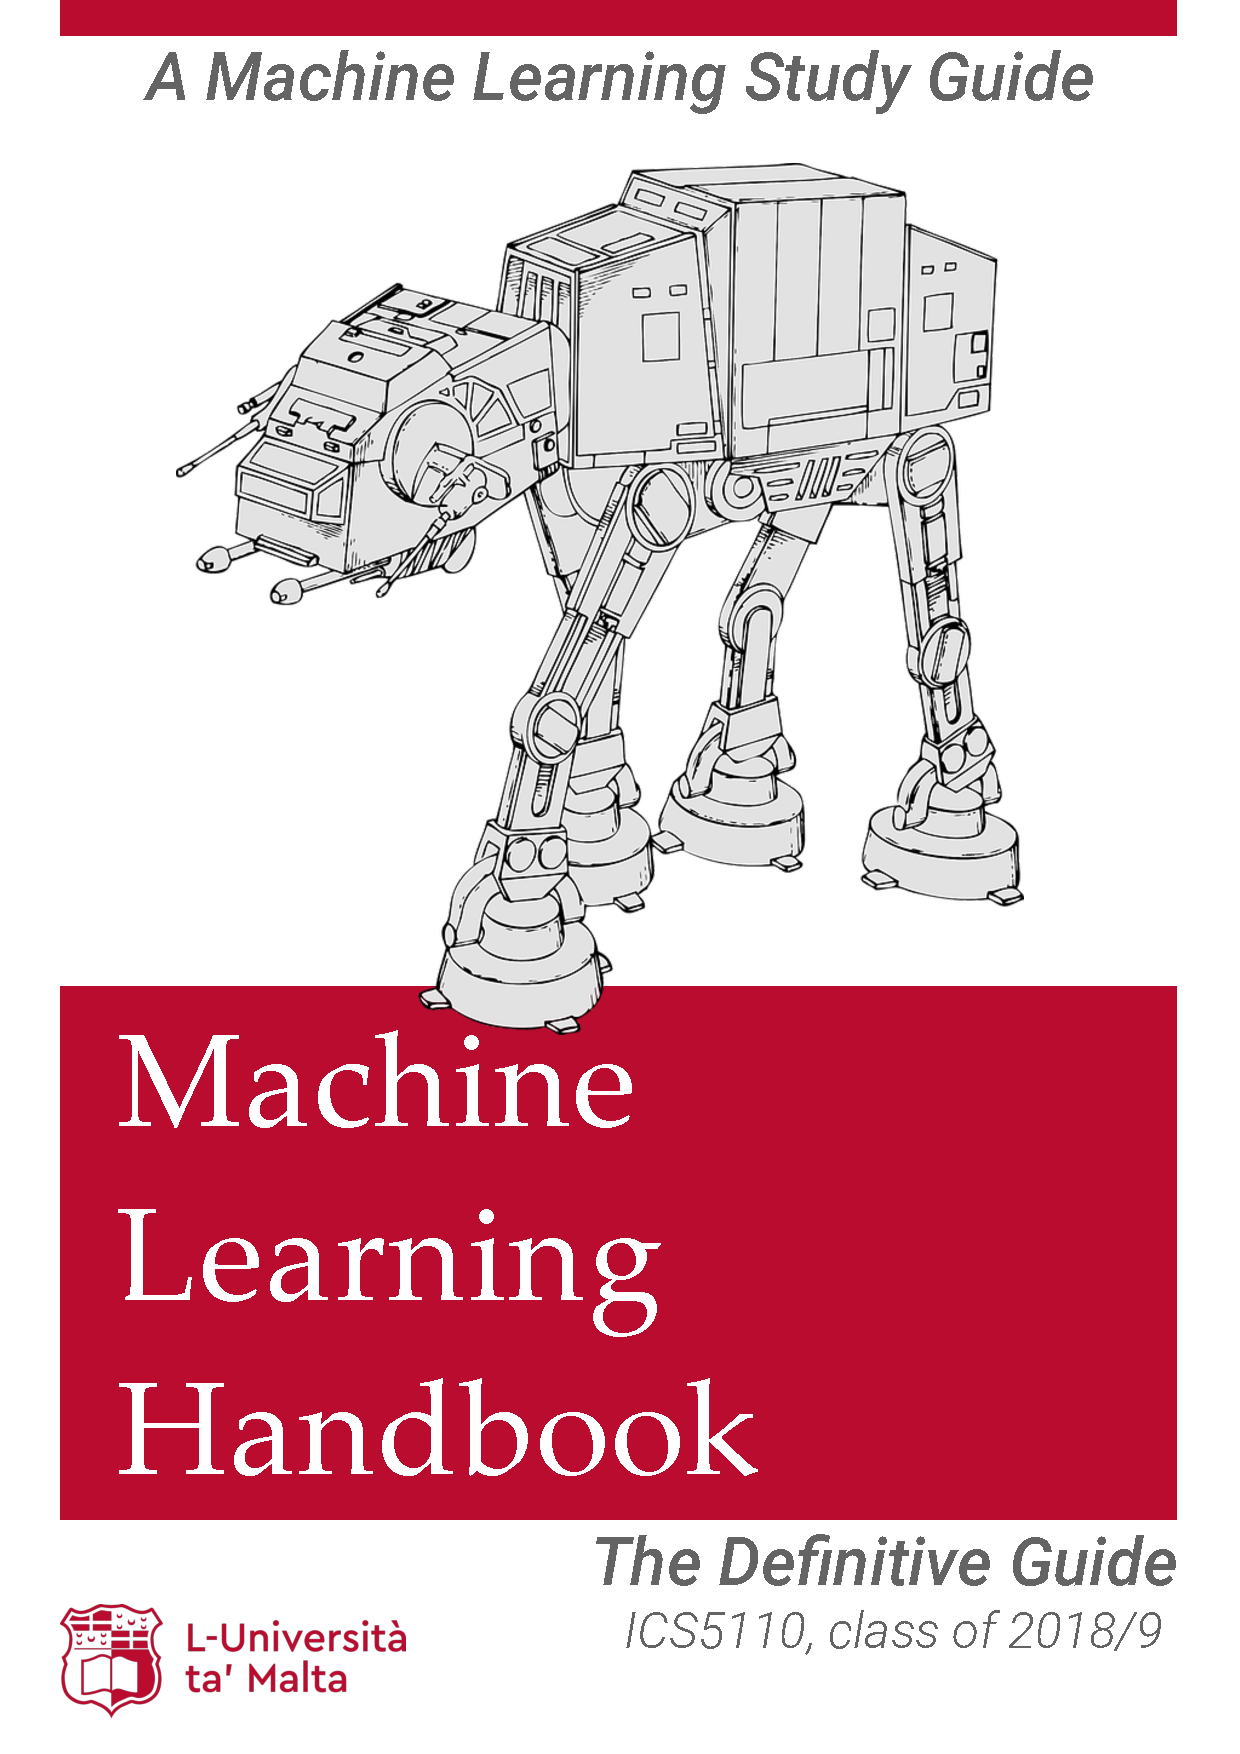
\includegraphics[width=\paperwidth]{cover/cover_oreilly_style.pdf}};
\end{tikzpicture}
\vfill
\endgroup

% Front matter
\frontmatter

% r.3 full title page
%% \maketitle


% v.4 copyright page
\newpage
\begin{fullwidth}
~\vfill
\thispagestyle{empty}
\setlength{\parindent}{0pt}
\setlength{\parskip}{\baselineskip}
\begin{figure*}[h]
	
\includegraphics[width=2.5in]{UMLOGO_redRGB.png}%
\end{figure*}

\par Copyright \copyright\ \the\year\ \ics\ class of 2018/9, University of Malta.

\par\smallcaps{Jean-Paul Ebejer, Dylan Seychell, Lara Marie Demajo, Daniel Farrugia, Keith Mintoff, George Eduardo Buckup Sulzbeck \hl{ADD YOUR NAME TO THIS LIST} } %TODO

\par Licensed under the Apache License, Version 2.0 (the ``License''); you may not
use this file except in compliance with the License. You may obtain a copy
of the License at \url{http://www.apache.org/licenses/LICENSE-2.0}. Unless
required by applicable law or agreed to in writing, software distributed
under the License is distributed on an \smallcaps{``AS IS'' BASIS, WITHOUT
WARRANTIES OR CONDITIONS OF ANY KIND}, either express or implied. See the
License for the specific language governing permissions and limitations
under the License.\index{license}

\par\textit{First printing, \monthyear}
\end{fullwidth}

% r.5 contents
\tableofcontents

%%\listoffigures

%%\listoftables

% r.9 introduction
\cleardoublepage
\chapter{Introduction}

This book explains popular Machine Learning terms.  We focus to explain each term comprehensively, through the use of examples and diagrams.  The description of each term is written by a student sitting in for \ics\footnote{\url{https://www.um.edu.mt/courses/studyunit/ICS5110}} at the University of Malta (class 2018/2019).  This study-unit is part of the MSc.\ in AI offered by the Department of Artificial Intelligence, Faculty of ICT.

%%
% Start the main matter (normal chapters)
\mainmatter

%% JP's example file -- file must be stored in directory "terms" and have
%% the term and initials of the student in the filename.
\chapter[Activation Functions]{Activation Functions}
\label{ch:activation-functions}\index{activation functions|(}
``Neural networks were originally conceived as a model that would imitate the function of the human brain---a set of neurons joined together by a set of connections. Neurons, in this context, are composed of a weighted sum of their inputs followed by a nonlinear function, which is also known as an activation function.'' \citep{caterini2018}

Activation Functions are used in Artificial Neural Networks to determine whether the output of the neuron should be considered further or ignored. If the activation function chooses to continue considering the output of a neuron, we say that the neuron has been activated. The output of the activation function is what is passed on to the subsequent layer in a multilayer neural network. To determine whether a neuron should be activated, the activation function takes the output of a neuron and transforms it into a value commonly bound to a specific range, typically from $0$ to $1$ or $-1$ to $1$ depending on the which activation function is applied.

\section{Step Function}\label{sec:step-function}\index{step function}

\begin{marginfigure}
  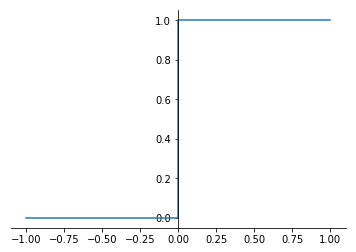
\includegraphics{graphics/activation_functions/step_function.png}
  \label{fig:stepfunction}
  \caption{
    A graph of the step function. 
  }
\end{marginfigure}

\begin{equation}\label{stepfunction}
    f(x) =
    \begin{dcases*}
        0 & \text{for \(x < 0\)} \\
        1 & \text{for \(x \geq 0\)} \\
    \end{dcases*}
\end{equation}

\begin{equation}\label{stepfunctionderivative}
    \frac{d}{d(x)}f(x) =
      \begin{dcases*}
                                       0 & \text{for \(x \neq 0\)} \\
                                       ? & \text{for \(x = 0\)} \\
      \end{dcases*}
\end{equation}

The Heavside step function, represented by Eq.~\ref{stepfunction}, is one of the simplest activation functions that can be used in a neural network. This activation function returns $0$ if the input of a node is less than a predetermined threshold (typically $0$), or otherwise it returns $1$ if the output of the node is greater than or equal to the threshold. This function was first used in a machine learning context in 1957 by Frank Rosenblatt in his seminal work describing the perceptron, the precursor to the modern day neural network \citep{rosenblatt1957perceptron}. 

Nowadays, the step function is seldom used in practice as it cannot be used to classify more than one class. Furthermore, since the derivative of this function, represented by Eq.~\ref{stepfunctionderivative}, is $0$, gradient descent algorithms are not be able to progressively update the weights of a network that makes use of this function \citep{Snyman2005}.

\section{Linear Functions}\label{sec:linear-function}\index{linear activation function}

A linear activation function seeks to solve some of the shortcomings of the step function. The output produced by a linear activation function is proportional to the input. While a linear activation function could be used for multi-class problems, it can on be used on problems that are linearly separable. Linear functions can also run into problems with gradient descent algorithms, as the derivative of a linear function is a constant. Additionally, since the output of the linear function is not bound to any range, it could be susceptible to a common problem when training deep neural networks called the exploding gradient problem, which can make learning unstable \citep{goodfellow2016deeplearning}.

\section{Sigmoid Function}\label{sec:sigmoid}\index{sigmoid function}

\begin{marginfigure}
  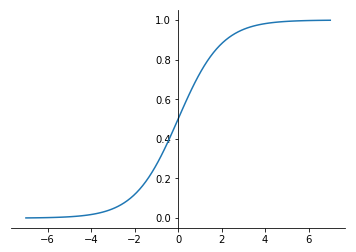
\includegraphics{graphics/activation_functions/sigmoid_function.png}
  \label{fig:sigmoidfunction}
  \caption{
    A graph of the sigmoid function.
  }
\end{marginfigure}

\begin{equation}\label{sigmoidfunction}
    f(x) = \frac{1}{(1 + e^{-x})}
\end{equation}

\begin{equation}\label{sigmoidfunctionderivative}
    \frac{d}{d(x)}f(x) = f(x)(1-f(x))
\end{equation}

The sigmoid function or logistic function, represented by  Eq.~\ref{sigmoidfunction}, is one of the most commonly used activation functions in neural networks, because of its simplicity and desirable properties. The use of this function in neural networks was first introduced by Rummelhart, Hinton and Williams in one of the most important papers in the field of machine learning, which described the back-propagation algorithm and the introduction of hidden layers, giving rise to modern day neural networks \citep{DavidE.Rumelhart1986Lrbb}.  The values produced by the step function are bound between $0$ and $1$, both not inclusive, which help manage the exploding gradient problem. The derivative of this function (Eq.~\ref{sigmoidfunctionderivative})  produces a very steep gradient for a relatively small range of values, typically in the range of $-2$ to $2$. This means that for most inputs that the function receives it will return values that are very close to either $0$ or $1$.

On the other hand, this last property makes the sigmoid function very susceptible to the vanishing gradient problem \citep{bengio94}. When observing the shape of the sigmoid function we see that towards the ends of the curve, function becomes very unresponsive to changes in the input. In other words, the gradient of the function for large inputs becomes very close to $0$. 

\section{Hyperbolic Tangent}\label{sec:tanh}\index{hyperbolic tangent}
\begin{marginfigure}
  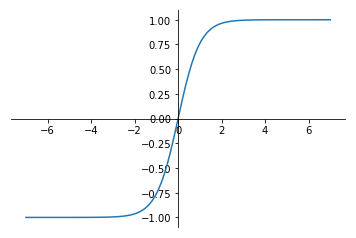
\includegraphics{graphics/activation_functions/tanh_function.png}
  \label{fig:tanhfunction}
  \caption{
    A graph of the hyperbolic tangent ($tanh$) function.
  }
\end{marginfigure}

\begin{equation}\label{tanhfunction}
    f(x) = \frac{(e^{x} - e^{-x})}{(e^{x} + e^{-x})}
\end{equation}

\begin{equation}\label{tanhfunctionderivative}
    \frac{d}{d(x)}f(x) = 1-f(x)^2.
\end{equation}

The hyperbolic tangent ($tanh$) function, represented by  Eq.~\ref{tanhfunction}, is another activation function that is sometimes used instead of sigmoid. The $tanh$ function has the same characteristics of the sigmoid function mentioned above. In fact the $tanh$ function is plotted, one can observe that it is simply a scaled version of the sigmoid function. As a result of this scaling, the tanh function has a steeper gradient in towards the origin, and it returns values between $-1$ and $1$. The derivative of the hyperbolic tangent function is represented by Eq.~\ref{tanhfunctionderivative}.

Nowadays with the rise of deep learning, these functions are becoming less commonly used. Xavier Glorot and Yoshua Bengio studied in detail the effects of the sigmoid and tanh activation functions. They note how the sigmoid function in particular is not well suited for deep networks with random initialization \citep{glorot2010understanding}.

\section{Rectified Linear Unit}\label{sec:relu}\index{rectified linear unit (relu)}
\begin{marginfigure}
  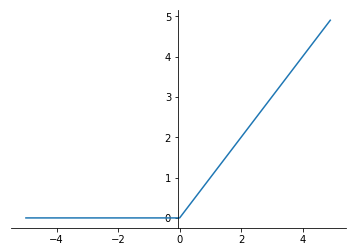
\includegraphics{graphics/activation_functions/relu_function.png}
  \label{fig:relufunction}
  \caption{
    A graph of the ReLU function.
  }
\end{marginfigure}

\begin{equation}\label{relufunction}
    f(x) =
      \begin{dcases*}
                                       0 & \text{for $x < 0$} \\
                                       x & \text{for $x \geq 0$} \\
      \end{dcases*}
\end{equation}

\begin{equation}\label{relufunctionderivative}
    \frac{d}{d(x)}f(x) =
      \begin{dcases*}
                                       0 & \text{for $x < 0$} \\
                                       1 & \text{for $x \geq 0$} \\
      \end{dcases*}
\end{equation}

The ReLU function, represented by  Eq.~\ref{relufunction}, returns $0$ if the input of the function is negative, otherwise it outputs the value of the input itself. This function is non-linear in nature even though at first glance it may seem similar to an identity function. The ReLU function is becoming one of the more commonly used activation function due to its simplicity performance, and suitability to networks with many layers. Another benefit of the ReLU function is that it produces sparse activations (not all nodes in the network are activated) unlike the sigmoid or hyperbolic tangent functions. 

The ReLU function has been used in many neural network models to improve their performance. Naid and Hinton use ReLU to improve the performance of Restricted Boltzmann Machines in object recognition \citep{Nair2010}. In 2012, a breakthrough Convolutional Neural Network (CNN) architecture called AlexNet pioneered the use of the ReLU activation function together with dropout layers to minimise over fitting in CNNs.  \citep{KrizhevskyAlex2017Icwd}. 

Unfortunately, because the gradient of the function for inputs that are negative is $0$ (Eq.~\ref{relufunctionderivative}), the ReLU function can still be susceptible to the vanishing gradient problem. To manage this problem a variant of the ReLU function, called Leaky ReLU is sometimes used. Rather than simply returning 0 for negative inputs, the leaky ReLU return a very small value such as $0.01x$. However, researchers at the University of Stanford compared the performance of Sigmoid, ReLU and Leaky ReLU functions and found that while the the performance of both the ReLU and Leaky Relu functions was better than the performance achieved with the sigmoid function, the performance of the two ReLU functions was nearly identical  \citep{maas2013rectifier}.
\index{activation functions|)}

\chapter{Confusion Matrix}
\label{ch:confusion-matrix}

A \textit{Confusion Matrix}\footnote{Also called a \textit{Contingency Table}.} (CM) is a cross-tabulation illustrating how well a model classifies categorical data. By convention \citep{sammut2017encyclopedia}, the CM of an N-class model is an N$\times$N matrix indexed by the true class in the row dimension and the predicted class in the column dimension (Table \ref{tab:cm_spam}).

\begin{table}[ht]
  \centering
  \fontfamily{ppl}\selectfont
  \begin{tabular}{llll}
    \toprule
                        &                     & \multicolumn{2}{c}{\textbf{Predicted Class}} \\
                        &                     & \textit{spam} & \textit{$\neg$spam} \\
    \midrule
    \textbf{True Class} & \textit{spam}       & 10           & 1 \\
                        & \textit{$\neg$spam} & 2            & 100 \\
    \bottomrule
  \end{tabular}
  \caption{CM of a hypothetical binary classifier which predicts whether out-of-sample text objects are spam or not. In this example, 10 spam and 100 non-spam objects are classified correctly, whilst 1 spam and 2 non-spam objects are misclassified.}
  \label{tab:cm_spam}
\end{table}

Even though CMs are commonly used to evaluate binary classifiers, they aren't restricted to 2-class models \citep{martin2018speech}. A CM of a multi-class model would show the number of times the classes were predicted correctly and which classes were confused with each other (Table \ref{tab:cm_sweets}).

\begin{table}[ht]
  \centering
  \fontfamily{ppl}\selectfont
  \begin{tabular}{llll}
    \toprule
                      & \textit{M\&M's} & \textit{Skittles} & \textit{Smarties} \\
    \midrule
    \textit{M\&M's}   & 34              & 3                 & 8  \\
    \textit{Skittles} & 1               & 28                & 5  \\
    \textit{Smarties} & 2               & 4                 & 22 \\
    \bottomrule
  \end{tabular}
  \caption{CM of a hypothetical sweets classifier. The main diagonal of the CM shows the number of correct predictions, whilst the remaining elements indicate how many sweets were misclassified.}
  \label{tab:cm_sweets}
\end{table}

The CM of the model $h : X \mapsto C$ over the concept $c : X \mapsto C$ using dataset $S \subset X$ is formally defined \citep{cichosz2014data} as a matrix $\Xi$ such that $\Xi_{c,S}(h)[d_1,d_2] = |S_{h=d_1,c=d_2}|$. The CM is constructed by incrementing the element corresponding to the true class \textit{vis-a-vi} the predicted class for each object in the dataset (Algorithm \ref{alg:cm}).

\begin{algorithm}
  \begin{algorithmic}
    \State $\Xi \gets 0$
    \For{$x \in S$}
      \State $d_1 \gets c(x)$
      \State $d_2 \gets h(x)$
      \State $\Xi_{d_1,d_2} \gets \Xi_{d_1,d_2} + 1$
    \EndFor
  \end{algorithmic}
  \caption{The CM is initialised to the zero matrix, and populated by iterating over all the objects $x$ with corresponding true class $d_1$ and predicted class $d_2$ and incrementing the element $(d_1,d_2)$ by 1 for each matching outcome.}
  \label{alg:cm}
\end{algorithm}

In binary classification, the CM consists of 2 specially designated classes called the \textit{positive} class and the \textit{negative} class \citep{saito2015precision}. As indicated in Table \ref{tab:cm_binary}, positive outcomes from the true class  which are classified correctly are called \textit{True Positives} (TP), whilst misclassifications are called \textit{False Negatives} (FN). On the other hand, negative true class outcomes which are classified correctly are called \textit{True Negatives} (TN), and misclassifications are called \textit{False Positives} (FP). In natural sciences, FP are called \textit{Type I Errors} and FN are known as \textit{Type II Errors} \citep{fielding1997review}.

\begin{table}[ht]
  \centering
  \fontfamily{ppl}\selectfont
  \begin{tabular}{lll}
    \toprule
                  & \textit{+ve} & \textit{-ve} \\
    \midrule
    \textit{+ve}  & TP           & FN \\
    \textit{-ve}  & FP           & TN \\
    \bottomrule
  \end{tabular}
  \caption{CMs of binary classifiers have positive (+ve) and negative (-ve) classes, and elements called \textit{True Positives} (TP), \textit{False Positives} (FP), \textit{True Negatives} (TN) and \textit{False Negatives} (FN).}
  \label{tab:cm_binary}
\end{table}

The information presented in the CM can be used to evaluate the performance of different binary classifiers \citep{lu2004predicting}. A number of statistics (Eq. \ref{eq:cm_acc}-\ref{eq:cm_fscore}) derived from the CM have been proposed in the literature \citep{deng2016improved} to gain a better understanding of what are the strengths and weaknesses of different classifiers. Caution should be exercised when interpreting metrics \citep{jeni2013facing}, since the CM could be misleading if the data is imbalanced and an important subrange of the domain (e.g. a rare diseases) is underrepresented \citep{raeder2012learning}.

These metrics are important in situations in which a particular type of misclassification, i.e. FP or FN, could have worse consequences than the other \citep{hassanien2017advances}. For example, FP are more tolerable than FN in classifiers which predict whether a patient has a disease or not. Even though both misclassifications are undesirable, in medical applications it's better to err on the side of caution since FN could be fatal.

\textit{Accuracy} (ACC) is the proportion of correct predictions (Eq. \ref{eq:cm_acc}). It is a class-insensitive metric because it can give a high rating to a model which classifies majority class objects correctly but misclassifies interesting minority class objects \citep{branco2016survey}. The other metrics should be preferred since they're more class-sensitive and give better indicators when the dataset is imbalanced.

\begin{equation}
\label{eq:cm_acc}
ACC = \frac{|TP \cup TN|}{|TP \cup FP \cup TN \cup FN|}
\end{equation}

\textit{Negative Predictive Value} (NPV) is the ratio of the correct negative predictions from the total negative predictions (Eq. \ref{eq:cm_npv}).

\begin{equation}
\label{eq:cm_npv}
NPV = \frac{|TN|}{|TN \cup FN|}
\end{equation}

\textit{True Negative Rate} (TNR), or \textit{Specificity}, is the ratio of the correct negative predictions from the total true negatives (Eq. \ref{eq:cm_tnr}).

\begin{equation}
\label{eq:cm_tnr}
TNR = \frac{|TN|}{|TN \cup FP|}
\end{equation}

\textit{True Positive Rate} (TPR), also called \textit{Sensitivity} or \textit{Recall}, is the ratio of the correct positive predictions from the total true positives (Eq.\ref{eq:cm_tpr}).

\begin{equation}
\label{eq:cm_tpr}
TPR = \frac{|TP|}{|TP \cup FN|}
\end{equation}

Sensitivity and Specificity can be combined into a single metric (Eq. \ref{eq:cm_ss}). These metrics are often used in  domains in which minority classes are important \citep{kuhn2013applied}. For example, a medical classifier \citep{el2010hybrid} could be evaluated by measuring Sensitivity to find the number of patients with a condition who tested positive, and Specificity to measure the number of patients who don't have the condition and tested negative.

\begin{equation}
\label{eq:cm_ss}
\textnormal{\textit{Sensitivity}} \times \textnormal{\textit{Specificity}} = \frac{|TP| \times |TN|}{|TP \cup FN| \times |TN \cup FP|}
\end{equation}

\textit{Positive Predictive Value} (PPV), or \textit{Precision}, is the ratio of the correct positive predictions from the total positive predictions (Eq. \ref{eq:cm_ppv}).

\begin{equation}
\label{eq:cm_ppv}
PPV = \frac{|TP|}{|TP \cup FP|}
\end{equation}

Precision and Recall are borrowed from the discipline of \textit{Information Extraction} \citep{sokolova2009systematic}. A composite metric called \textit{F-score}, \textit{F1-score}, or \textit{F-measure} (Eq. \ref{eq:cm_fscore}) can be derived by finding their harmonic mean \citep{kelleher2015fundamentals}.

\begin{equation}
\label{eq:cm_fscore}
\textnormal{\textit{F-score}} = 2 \times \frac{PPV \times TPR}{PPV + TPR}
\end{equation}

The complements of ACC, NPV, TNR, TPR and PPV are called, respectively, \textit{Error Rate}, \textit{False Omission Rate}, \textit{False Positive Rate}, \textit{False Negative Rate} and \textit{False Discovery Rate}.

Using all metrics could be counterproductive due to information redundancy, but none of the metrics is enough on its own \citep{ma2007adequate}. For instance, Recall is class-sensitive but it would give a perfect score to an inept model which simply returns the positive class. Thus, the best approach is to evaluate with complementary pairs \citep{gu2009evaluation} such as Sensitivity \textit{vs.} Specificity, or Precision \textit{vs.} Recall; or a combined measure such as the F-score.

The metrics can be adapted for evaluating multi-class models by decomposing an N-class CM into 2-class CMs, and evaluating them individually \citep{stager2006dealing}. The literature describes two methods for decomposing this kind of  CM. In the \textit{1-vs-1} approach, 2-class CMs are constructed for each pairwise class as shown in Table \ref{tab:cm_1vs1}.

\begin{table}[ht]
  \centering
  \fontfamily{ppl}\selectfont
  \begin{tabular}{ll}
    \toprule
    \textit{+ve} & \textit{-ve} \\
    \midrule
    M\&M's       & $\{$Skittles, Smarties$\}$ \\
    Skittles     & $\{$M\&M's, Smarties$\}$ \\
    Smarties     & $\{$M\&M's, Skittles$\}$ \\
    \bottomrule
  \end{tabular}
  \caption{2-class CMs derived from the classes in Table \ref{tab:cm_sweets}. The +ve classes are paired separately with each -ve class.}
  \label{tab:cm_1vs1}
\end{table}

In the \textit{1-vs-rest} approach, 2-class CMs are constructed for each class and the remaining classes combined together as shown in Table \ref{tab:cm_1vsN}.

\begin{table}[ht]
  \centering
  \fontfamily{ppl}\selectfont
  \begin{tabular}{ll}
    \toprule
    +ve       & -ve \\
    \midrule
    M\&M's    & Skittles $\cup$ Smarties \\
    Skittles  & M\&M's $\cup$ Smarties \\
    Smarties  & Skittles $\cup$ M\&M's \\
    \bottomrule
  \end{tabular}
  \caption{2-class CMs derived through decomposition of the 3-class CM from Table \ref{tab:cm_sweets} using the 1-vs-rest approach.}
  \label{tab:cm_1vsN}
\end{table}

Taking into account the above, CMs are suitable for visualising, evaluating, and comparing the performance of binary or multi-class classifiers. They should be used in conjunction with metrics such as the F-measure to avoid bias, especially if the dataset is unbalanced. For further details on the theoretical aspects of CMs and for practical examples in R refer to \citep{cichosz2014data}; for examples in Python refer to \citep{muller2016introduction}.

The following example is motivated by the samples in the \textit{Scikit-Learn} documentation and the work of  \citep{geron2017hands}. The models in Fig. \ref{fig:cm_model} were trained on 70\% of the \textit{wines} dataset included with Scikit-Learn, whilst the remaining 30\% was kept as a test set to evaluate the model. The dataset has 3 classes and 13 features, but only the results for class 1 and 2; and the alcohol and malic acid features; will be presented. It was scaled by standardising the features using $\frac{x_i - \mu}{\sigma}$, for all $x_i \in S$ using mean $\mu$ and standard deviation $\sigma$.

\begin{figure}
  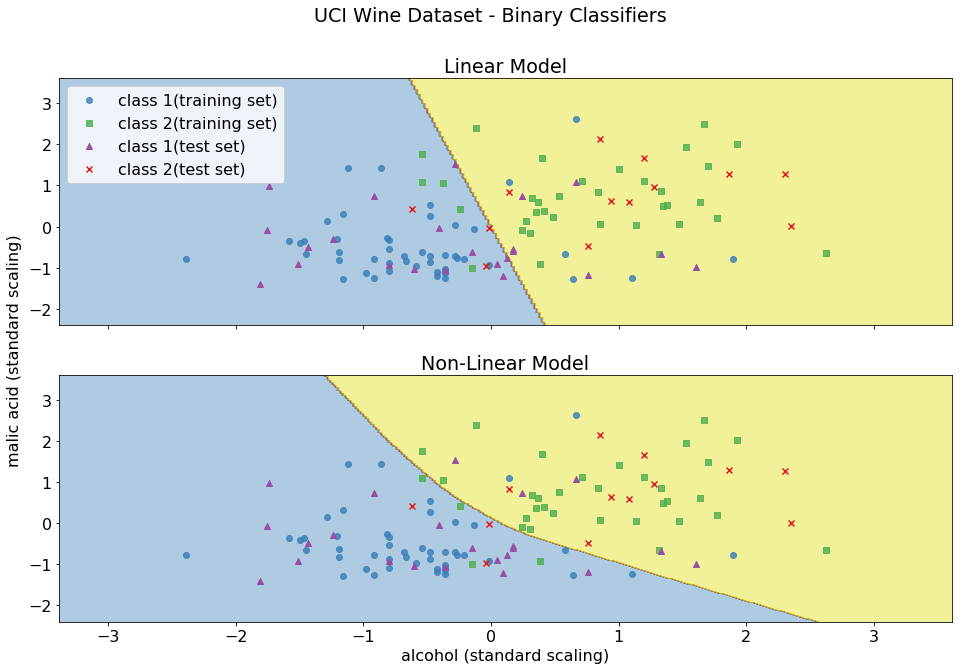
\includegraphics{confusion_matrix/model.png}
  \caption{Decision boundary learned by a linear and non-linear binary classifier.}
  \label{fig:cm_model}
\end{figure}

\begin{margintable}
  \begin{tabular}{lll}
    \toprule
                 & Linear & Non-Linear \\
    \midrule
    Accuracy     & 0.72   & 0.78 \\
    Specificity  & 0.77   & 0.77 \\
    Sensitivity  & 0.70   & 0.78 \\
    Precision    & 0.84   & 0.86 \\
    F-score      & 0.76   & 0.82 \\
    \bottomrule
  \end{tabular}
  \caption{Statistics derived from the CMs in Fig. \ref{fig:cm_wines}.}
  \label{tab:cm_metrics}
\end{margintable}

As it can be intuitively deduced from Fig. \ref{fig:cm_model}, the decision boundary of the non-linear model is a better fit than the linear model. The CMs in Fig. \ref{fig:cm_wines} also show that non-linear model performs better with a higher TP, and consequently lower TN. The biggest advantage of the non-linear model is the higher Sensitivity resulting in a better F-score.

\begin{figure}
  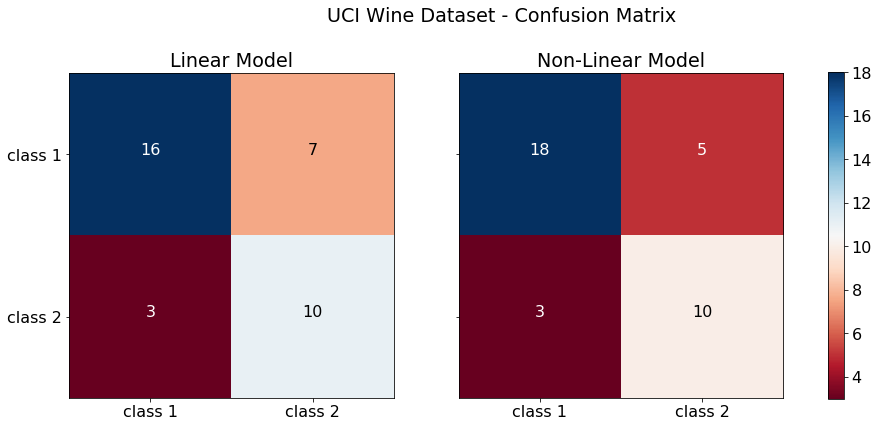
\includegraphics{confusion_matrix/cm.png}
  \caption{The linear classifier has 16 TP, 10 TN, 7 FN and 3 FP, whilst the non-linear classifier has 18 TP, 10 TN, 5 FN and 3 FP.}
  \label{fig:cm_wines}
\end{figure}

\index{class options|)}

\chapter[Convolution]{Convolution}
\label{ch:convolution}
\index{convolution in mathematics|(}
\section{Convolution in Mathematics}
\label{sec:convolution:mathematics}
\subsection{Definition}
\label{sec:convolution:mathematics:definitions}
\index{definition!convolution in mathematics}
Convolution is a mathematical operation on two functions to produce a result that reflects how one of the input functions is modified by the other input function.\newline
The convolution of functions $f(x)$ and $g(x)$ (denoted $f*g(x)$) is defined  \citep{Bracewell2000}, for continuous functions $f$ and $g$, as\footnote{In order for the continuous convolution operator $f * g$ to be defined, both $f$ and $g$ must be integrable functions.}
\begin{equation}
(f * g) (t)\equiv\int_{-\infty}^{\infty} f(\tau) g(t-\tau)d\tau
\end{equation}
\begin{figure*}[h]
    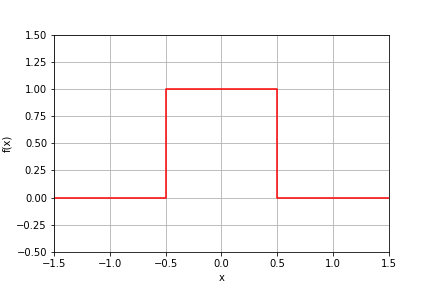
\includegraphics[width=.32\linewidth]{graphics/convolution/convolution_continuos_f_gebs.png}
    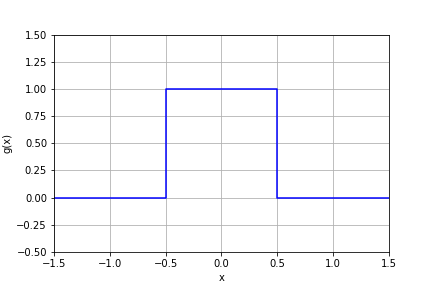
\includegraphics[width=.32\linewidth]{graphics/convolution/convolution_continuos_g_gebs.png}
    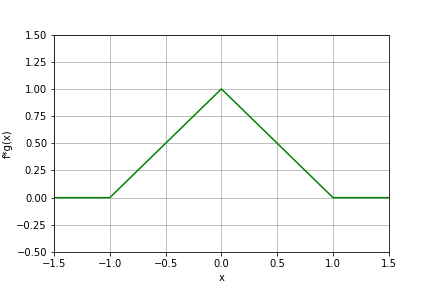
\includegraphics[width=.32\linewidth]{graphics/convolution/convolution_continuos_fg_gebs.png}
    \caption{These plots show two continuous functions ($f(x)$ and $g(x)$) and their convolution $f*g(x)$}.
    \label{fig:continuousconvolution}
\end{figure*}\FloatBarrier
and, for discrete functions $f(n)$ and $g(n)$, as
\begin{equation}
(f * g)(n)\equiv\sum_{m=-\infty}^{\infty}f(m) g(n-m)
\end{equation}
\begin{figure*}[h]
    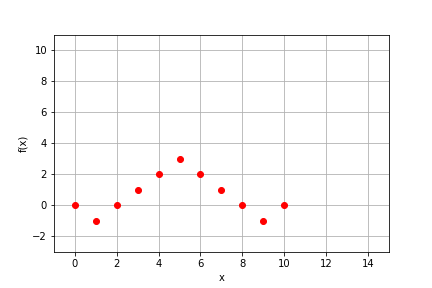
\includegraphics[width=.32\linewidth]{graphics/convolution/convolution_discrete_f_gebs.png}
    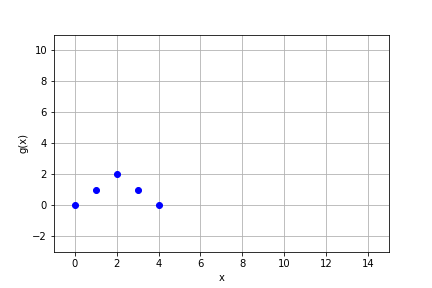
\includegraphics[width=.32\linewidth]{graphics/convolution/convolution_discrete_g_gebs.png}
    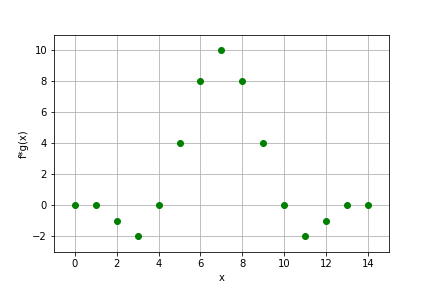
\includegraphics[width=.32\linewidth]{graphics/convolution/convolution_discrete_fg_gebs.png}
    \caption{These plots show two discrete functions ($f(n)$ and $g(n)$) and their convolution $f*g(n)$}.
    \label{fig:discreteconvolution}
\end{figure*}\FloatBarrier
\subsection{Properties}
\label{sec:convolution:mathematics:properties}
\index{properties!convolution in mathematics}
Since convolution is defined as a product of integrable functions on the linear space, the following algebraic properties are satisfied \citep{Bracewell2000}:\newline
\textbf{Commutativity}
\begin{equation}
(f * g)=(g * f)
\end{equation}
\textbf{Associativity}
\begin{equation}
(f * (g * h))=((f * g) * h)
\end{equation}
\textbf{Distributivity}
\begin{equation}
(f * (g + h))=(f * g) + (f * h)
\end{equation}
\textbf{Multiplication by a scalar value}
\begin{equation}
a (f * g) = (af) * g
\end{equation}
\textbf{Multiplicative identity}, where $\delta$ denotes the delta distribution 
\begin{equation}
f * \delta = f
\end{equation}
\textbf{Differentiation}
\begin{equation}
\frac{d}{dx}(f * g) = \frac{df}{dx} * g = f * \frac{dg}{dx}
\end{equation}
\textbf{Integration}
\begin{equation}
\int_{R^d} (f * g)(x)dx = \bigg(\int_{R^d} f(x)dx\bigg)\bigg(\int_{R^d} g(x)dx\bigg)
\end{equation}
\subsection{Applications}
\label{sec:convolution:mathematics:applications}
\index{applications!convolution in mathematics}
Listed below are some of the main applications of the convolution operator in various fields of knowledge \citep{Srivastava2013}:
\begin{itemize}
	\item \textbf{Image Processing} - Different operations are performed on images, in which the original image (larger matrix) and the filter to be applied (smaller matrix, also known as 2D kernel) are treated as 2-dimensional arrays. The kernel size and the values of its elements determine the effect on the original image
    \item \textbf{Signal Filtering} - Provided the filter function is the same as the impulse response function used in in signal filtering, the two operations are equivalent
    \item As a handy tool for \textbf{Polynomial Multiplication} - If we consider two polynomials being multiplied, we can use a convolution process to obtain the coefficients of the resulting polynomial
    \item \textbf{Audio Processing} - Reverberation is a desired effect in auditoriums, music halls, cinemas, and similar constructions. Convolution is used to digitally simulate reverberation in such structures, providing architects with information about the acoustic quality of a building prior to its construction
    \item \textbf{Artificial Intelligence} - Convolutional Neural Networks use convolution in one or more of its internal layers in order to process input data and enhance specific features.
    \item \textbf{Probability Theory} - The Probability Density Function (PDF) of the sum of two independent random variables can be obtained by the convolution of the PDFs of the two variables
\end{itemize}
\index{convolution in mathematics|)}
\index{convolutional neural networks|(}
\section{Convolution in Neural Networks}
\label{sec:convolution:convolutionalneuralnetworks}
\index{definition!convolutional neural networks}
\subsection{Definition}
\label{sec:convolution:convolutionalneuralnetworks:definition}
A Convolutional Neural Networks (CNNs) are a subclass of multi-layer neural networks in which some of its hidden layers are convolutional layers.\newline
Like most neural networks, CNNs can be trained using back-propagation algorithms and are mostly used to recognize visual patters with minimal or no preprocessing \citep{Lawrence1997A}.\newline
\index{origins and evolution!convolutional neural networks}
\subsection{Origins and Evolution}
\label{sec:convolution:convolutionalneuralnetworks:originsandevolution}
CNNs were initially developed as an attempt to replicate the processing of sight in living organisms.\newline
A seminal paper published in 1968 \citep{Hubel1968} noted that two types of neurons took part in the process of identifying images: simple cells (responsible for the detection of straight edges and their orientation), and complex cells (with larger receptive fields, but not affected by the exact position of the edges in the input image).\newline
During the 1980s, CNNs evolved, followed by the introduction of Time Delay Neural Networks (TDNNs) in 1987 \citep{Waibel1989}.\newline
In the early 1990s, CNNs were modified and used for medical image processing and for automatic detection of breast cancer in mammograms \citep{Zang1994}.\newline
In 1998 LeCun lead a team that created LeNet-5, a CNN used by banks to identify handwritten digits in checks.\newline
With the introduction of Graphic Processing Units (GPUs), training of CNNs was greatly improved, allowing for the implementation of efficient Deep Learning Neural Networks with impressive results in image processing and other applications  \citep{Ciresan2013}.
\index{layers!convolutional neural networks}
\subsection{Layers}
\label{sec:convolution:convolutionalneuralnetworks:layers}
A typical CNN has sets of layers with specific functions, such as:
\begin{itemize}
    \item \textbf{Convolutional layer} - This is the main feature of a CNN.\newline
    In this layer, a set of filters (also known as kernels) is convoluted over the entire input data. The result of this operation (the activation map of the filter), extracts or enhances specific features in the input data that are passed to the following layers in the CNN.\newline
    Since the result of each convolution operation is affected by only a small part of the input data (due to the reduced size of the filter if compared to the size of the input data), this can be interpreted as each point of the activation map being affect by only a small subset of input points.
    \item \textbf{Pooling layer} - In this layer, simple operations are applied in order to reduce the size of the input data, such as maximum pooling or average pooling.\newline
    In 2x2 average pooling, for example, each result point the the average of 4 input points, reducing the size of the input field by a factor of 4.
    \item \textbf{Rectified Linear Unit (ReLU) layer} - This layer applies the $f(x) = max(0,x)$ activation function to its input, removing negative values from the input field.
    \item \textbf{Fully Connected layer} - In this layer, usually applied after several convolutional and pooling layers, neurons are connected to all activations in the previous layer, as in regular neural networks.
    \item \textbf{Loss layer} - This is the last layer in a typical CNN. In this layer, training is based on the divergence between the desired and predicted labels.
\end{itemize}
\index{training!convolutional neural networks}
\subsection{Training}
\label{sec:convolution:convolutionalneuralnetworks:training}
One important feature of CNNs is that, with the exception of the Loss layer, all other layers (Convolutional, Pooling, ReLU, and Fully Connected layers) can be trained using unsupervised training  \citep{Arel2010}.\newline
Also, usually each layer or set of layers is trained individually, which also improves the speed and the overall result of the training.\newline
With the introduction of Graphic Processing Units (GPUs), speed of training and processing in the Convolutional layer has been greatly improved  \citep{Steinkrau2005}
\index{applications!convolutional neural networks}
\subsection{Applications}
\label{sec:convolution:convolutionalneuralnetworks:applications}
CNNs are currently applied to a wide range of areas, such as  \citep{Schmidhuber2015}:
\begin{itemize}
    \item \textbf{Image recognition and Video analysis} - Image Recognition Systems using CNNs are very efficient, specially if applied to facial recognition. Very good results have been obtained in challenges, and in the ImageNetNet tests performed almost as good as humans. If compared to image recognition, video analysis adds a level of complexity, since, in addition to the analysis of each frame, a time dimension needs to be added to the problem and convolution needs to be performed both on each image as well as on the time domain.
    \item \textbf{Game strategy} - A number of board games have been implements using CNNs, most notably Checkers, in Chess and in Go, the first time Artificial Intelligence beat an expert human player in this game.
    \item \textbf{Drug discovery} - In this area, CNNs are used to predict the behaviour of drug molecules and human proteins.
    \item \textbf{Natural language processing} - For NLP, CNNs are used extensively, including semantic parsing, search query retrieval, sentence modeling, classification, and prediction.
\end{itemize}
\clearpage
\index{convolutional neural networks|)}
\index{convolutional filters|(}
\section{Convolutional Filters}
\label{sec:convolution:convolutionalfilters}
\index{definition!convolutional filters}
\subsection{Definition}
\label{sec:convolution:convolutionalfilters:definition}
Convolutional filters (also known as kernels), when applied to image and video processing, are small square matrices with an odd number of rows and columns and used in the Convolutional layer of CNNs in order to detect or enhance specific features in the input image.\newline
The convolution operation performed by CNNs is a special two dimensional case of the discrete convolution operator.
\begin{equation}
R(m,n) = (K * I)(m,n)\equiv\sum_{s=-a}^{a}\sum_{t=-b}^{b}K(s,t)I(m-s,n-t)
\end{equation}
where $R(m,n)$ is the convoluted result at point $m,n$, $K$ is the kernel matrix being applied to the input matrix, $I$ is the input matrix, and $a$ and $b$ depend on the dimensions of the kernel used.
\index{common convolutional filters!convolutional filters}
\subsection{Common Convolutional Filters}
\label{sec:convolution:convolutionalfilters:commonconvolutionalfilters}
Convolutional filters can be defined to achieve a large range of effects in the input image.\newline
A small sample of possible kernels is provided below:\newline
\begin{itemize}
    \item \textbf{Identity} - This is the input image, without any convolution applied.
    $$
    \quad
    \begin{bmatrix} 
    0 & 0 & 0 \\
    0 & 1 & 0 \\
    0 & 0 & 0
    \end{bmatrix}
    $$
    \begin{center}
	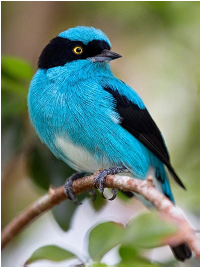
\includegraphics[width=1in]{graphics/convolution/Convolution_gebs_KernelIdentity.png}
    \end{center}
    \item \textbf{Gaussian blur}
    $$
    \frac{1}{16}
    \quad
    \begin{bmatrix} 
    1 & 2 & 1 \\
    2 & 4 & 2 \\
    1 & 2 & 1
    \end{bmatrix}
    $$
    \begin{center}
	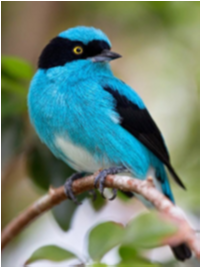
\includegraphics[width=1in]{graphics/convolution/Convolution_gebs_KernelGaussianBlur3x3.png}
    \end{center}
    \item \textbf{Box blur}
    $$
    \frac{1}{9}
    \quad
    \begin{bmatrix} 
    1 & 1 & 1 \\
    1 & 1 & 1 \\
    1 & 1 & 1
    \end{bmatrix}
    $$
    \begin{center}
	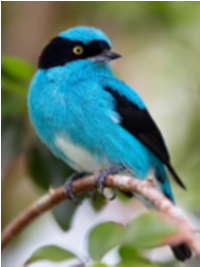
\includegraphics[width=1in]{graphics/convolution/Convolution_gebs_KernelBoxBlur.png}
    \end{center}
    \item \textbf{Unsharp}
    $$
    \frac{-1}{256}
    \quad
    \begin{bmatrix} 
    1 & 4 & 6 & 4 & 1 \\
    4 & 16 & 24 & 16 & 4 \\
    6 & 24 & -476 & 24 & 6 \\
    4 & 16 & 24 & 16 & 4 \\
    1 & 4 & 6 & 4 & 1
    \end{bmatrix}
    $$
    \begin{center}
	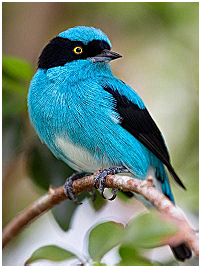
\includegraphics[width=1in]{graphics/convolution/Convolution_gebs_KernelUnsharp5x5.png}
    \end{center}
    \item \textbf{Sharpen}
    $$
    \quad
    \begin{bmatrix} 
    0 & -1 & 0 \\
    -1 & 5 & -1 \\
    0 & -1 & 0
    \end{bmatrix}
    $$
    \begin{center}
	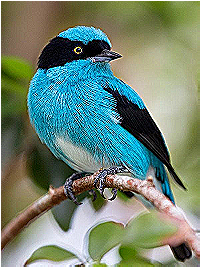
\includegraphics[width=1in]{graphics/convolution/Convolution_gebs_KernelSharpen.png}
    \end{center}
    \item \textbf{Edge detection}
    $$
    \quad
    \begin{bmatrix} 
    -1 & -1 & -1 \\
    -1 & 8 & -1 \\
    -1 & -1 & -1
    \end{bmatrix}
    $$
    \begin{center}
	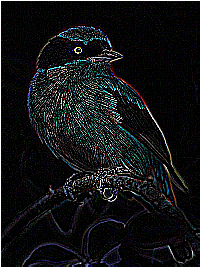
\includegraphics[width=1in]{graphics/convolution/Convolution_gebs_KernelEdgeDetection.png}
    \end{center}
\end{itemize}
\index{convolutional filters|)}

\chapter{\textit{}Cross-Validation}
\label{ch:cross-validation}\index{cross-validation}

Cross-validation (CV) is an estimation method used on supervised learning algorithms to assess their ability to predict the output of unseen data \cite[-3\baselineskip]{varma2006bias,kohavi1995study}. Supervised learning algorithms are computational tasks like classification or regression, that learn an input-output function based on a set of samples. Such samples are also known as the labeled training data where each example consists of an input vector and its correct output value. After the training phase, a supervised learning algorithm should be able to use the inferred function in order to map new input unseen instances, known as testing data, to their correct output values \cite{caruana2006empirical}. When the algorithm incorporates supervised feature selection, cross-validation should always be done external to the selection (feature-selection performed within every CV iteration) so as to ensure the test data remains unseen, reducing bias \cite[-3\baselineskip]{ambroise2002selection, friedman2001elements}.  Therefore, cross-validation, also known as out-of-sample testing, tests the function's ability to generalize to unseen situations \cite[-3\baselineskip]{varma2006bias,kohavi1995study}. 

Cross-validation has two types of approaches, being i) the exhaustive cross validation approach which divides all the original samples in every possible way, forming training and test sets to train and test the model, and ii) the non-exhaustive cross validation approach which does not consider all the possible ways of splitting the original samples \cite{arlot2010survey}. Each of these approaches are further divided into different cross-validation methods, which are explained below.
\\\\
\noindent\textbf{Exhaustive cross-validation}
\begin{itemize}
\item Leave-$p$-out (L$p$O) \newline \index{leave-p-out}
This method takes $p$ samples from the data set as the test set and keeps the remaining as the training set, as shown in Fig.~\ref{fig:leavep}a. This is repeated for every combination of test and training set formed from the original data set and the average error is obtained. Therefore, this method trains and tests the algorithm $n\choose p$ times when the number of samples in the original data set is $n$, becoming inapplicable when $p>1$ \cite{arlot2010survey}.

\item Leave-one-out (LOO)\newline \index{leave-one-out}
This method is a specific case of the LpO method having $p=1$. It requires less computation efforts than LpO since the process is only repeated $n choose 1$ $= n$ times, however might still be inapplicable for large values of $n$ \cite{arlot2010survey}. 
\end{itemize}

\begin{figure*}
\centering
\begin{subfigure}
  \centering
  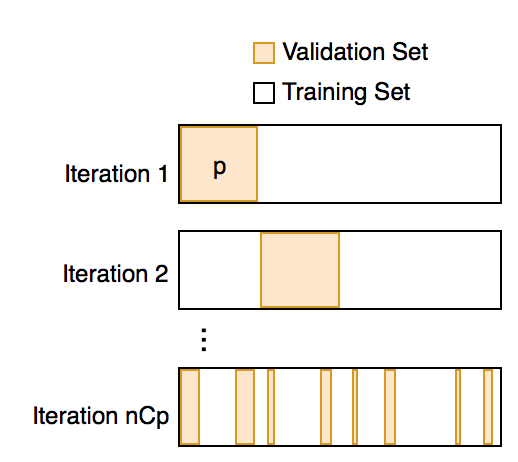
\includegraphics[width=.4\linewidth]{leavep.png}
  \caption{Leave-p-Out}
  \end{subfigure}
 \begin{subfigure}
  \centering
  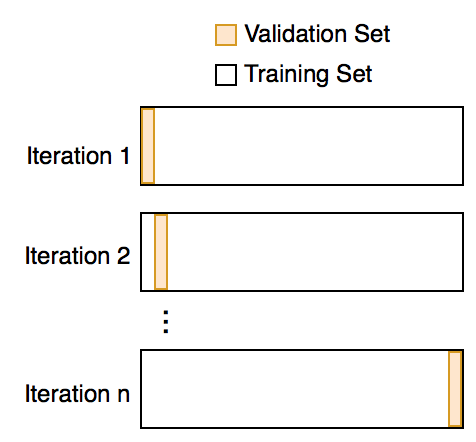
\includegraphics[width=.37\linewidth]{leave1.png}
  \caption{Leave-One-Out}
  \end{subfigure}
  \caption{Exhaustive cross-validation methods: Leave-p-Out (left) \& Leave-One-Out (right)}
  \label{fig:leavep}
\end{figure*}

\break\noindent\textbf{Non-exhaustive cross-validation}
\begin{itemize}
\item Holdout method \newline \index{holdout}
This method randomly splits the original data set into two sets being the training set and the test set. Usually, the test set is smaller than the training set so that the algorithm has more data to train on. This method involves a single run and so must be used carefully to avoid misleading results. It is therefore sometimes not considered a CV method \cite{kohavi1995study}.

\item $k$-fold\newline \index{k-fold}
This method randomly splits the original data set into $k$ equally sized subsets, as shown in Fig.~\ref{fig:kfold}. The function is then trained and validated $k$ times, each time taking a different subset as the test data and the remaining $(k-1)$ subsets as the training data, using each of the $k$ subsets as the test set once. The $k$ results are averaged to produce a single estimation. Stratified $k$-fold cross validation is a refinement of the $k$-fold method, which splits the original samples into equally sized and distributed subsets, having the same proportions of the different target labels \cite{kohavi1995study}.

\begin{figure}
\centering
  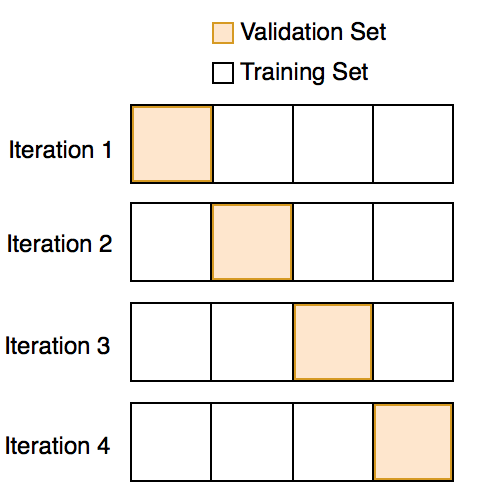
\includegraphics[width=0.5\linewidth]{kfold.png}
  \caption{$k$-Fold Cross Validation where $k$=4}
  \label{fig:kfold}
\end{figure}

\item Repeated random sub-sampling\newline \index{repeated random sub-sampling}
This method is also known as the Monte Carlo CV. It splits the data set randomly with replacement into training and test subsets using some predefined split percentage, for every run. Therefore, this generates new training and test data for each run but the test data of the different runs might contain repeated samples, unlike that of $k$-fold \cite{xu2001monte}.
\end{itemize}

All of the above cross-validation methods are used to check whether the model has been overfitted or underfitted and hence estimating the model's ability of fitting to independent data . Such ability is measured using quantitative metrics appropriate for the model and data \cite[-3\baselineskip]{kohavi1995study, arlot2010survey}. In the case of classification problems, the misclassification error rate is usually used whilst for regression problems, the mean squared error (MSE) is usually used. MSE is represented by Eq.~\ref{mse}, where n is the total number of test samples, $Y_i$ is the true value of the $i^{th}$ instance and $\hat{Y}_i$ is the predicted value of the $i^{th}$ instance.

\begin{equation}\label{mse}
MSE = \frac{1}{n}\sum^{n}_{i=1}(Y_i - \hat{Y}_i)^2
\end{equation}

Underfitting \index{underfitting} is when the model has a low degree (e.g. $y = x$, where the degree is 1) and so is not flexible enough to fit the data making the model have a low variance and high bias \cite{baumann2003cross}, as seen in Fig.~\ref{fig:models}a. Variance is the model's dependence on the training data and bias is model's assumption about the shape of the data \cite{arlot2010survey}. On the other hand, as seen in Fig.~\ref{fig:models}b, overfitting \index{overfitting} is when the model has a too high degree (e.g. $y = x^{30}$, where the degree is 30) causing it to exactly fit the data as well as the noise and so lacks the ability to generalize \cite{baumann2003cross}, making the model have a high variance. Cross-validation helps reduce this bias and variance since it uses most of the data for both fitting and testing and so helps the model learn the actual relationship within the data. This makes cross-validation a good technique for models to acquire a good bias-variance tradeoff \cite{arlot2010survey}.

\begin{figure*}
\centering
\begin{subfigure}
  \centering
  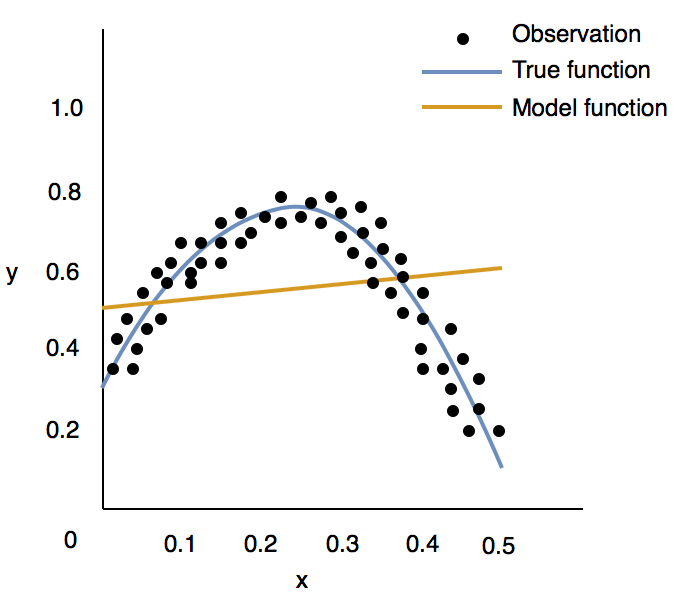
\includegraphics[width=0.4\linewidth]{underfitting.png}
  \caption{Underfitting}
  \label{fig:underfitting}
\end{subfigure}
\begin{subfigure}
  \centering
  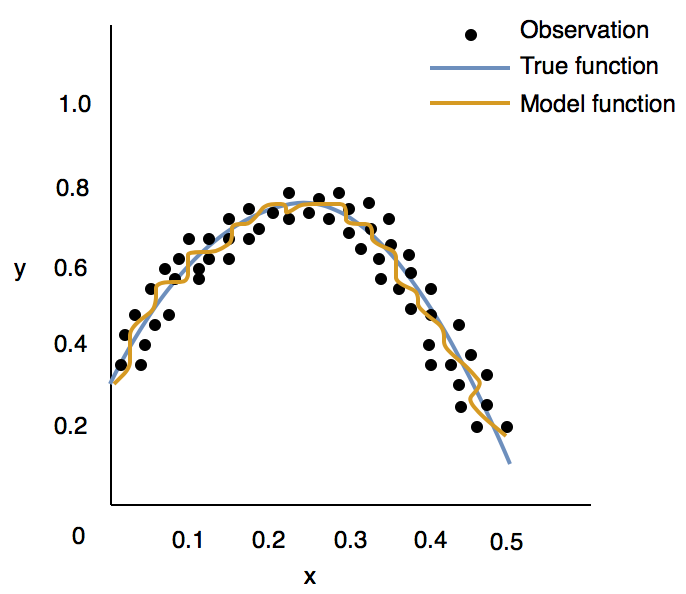
\includegraphics[width=.4\linewidth]{overfitting.png}
  \caption{Overfitting}
  \label{fig:overfitting}
\end{subfigure}
\caption{Underfitting (left) \& Overfitting (right)}
\label{fig:models}
\end{figure*}

As stated in \cite{kohavi1995study}, the LOO method gives a 0\% accuracy on the test set when the number of target labels are equal to the number of instances in the dataset. It is shown that the $k$-fold CV method gives much better results, due to its lower variance, especially when $k = {10, 20}$. Furthermore, R. Kohavi et al. state that the best accuracy is achieved when using the stratified cross-validation method, since this has the least bias.

Therefore, lets take an example using the stratified $k$-fold cross-validation method with $k=10$. Let's say that we are trying to solve age group classification, using eight non-overlapping age groups being 0-5, 6-10, 11-20, 21-30, 31-40, 41-50, 51-60, and 61+. We are using the FG-NET labelled data set, which contains around 1000 images of individuals aged between 0 and 69. Before we can start training our model (e.g. CNN), we must divide our data set into training and test subsets and this is where cross validation comes in. Therefore, we start by taking the 1000 images of our data set and splitting them according to their target class. Let us assume we have an equal amount of 125 $(1000/8)$ images per class\footnote{Down-sampling or up-sampling are common techniques used when there is an unequal amount of samples for the different classes.}. As depicted in Fig.~\ref{fig:example}, we can now start forming our 10 folds by taking 10\% of each age-group bucket, randomly without replacement. Hence, we will end up with 10 subsets of 100 images that are equally distributed along all age-groups. With these subsets, we can estimate our model's accuracy with a lower bias-variance tradeoff. Since we are using 10-fold CV, we will train and test our model 10 times. For the first iteration, we shall use subset 1 as the validation set and subsets 2 to 10 as the training set, for the second iteration we use subset 2 as the test set and subsets 1 plus 3 to 10 as our training set, and so on (as shown in Fig.~\ref{fig:kfold}). For each iteration we use the misclassification error rate to obtain an accuracy value and we finally average the 10 accuracy rates to obtain the global accuracy of our model when solving age group classification, given the FG-NET data set. Hence, we have now estimated the prediction error of the model and have an idea of how well our model performs in solving such a problem. It is important to note that cross-validation is \textit{just} an estimation method and when using our model in real-life applications we do not apply CV but rather train our model with all the data we have.

\begin{figure*}
\centering
  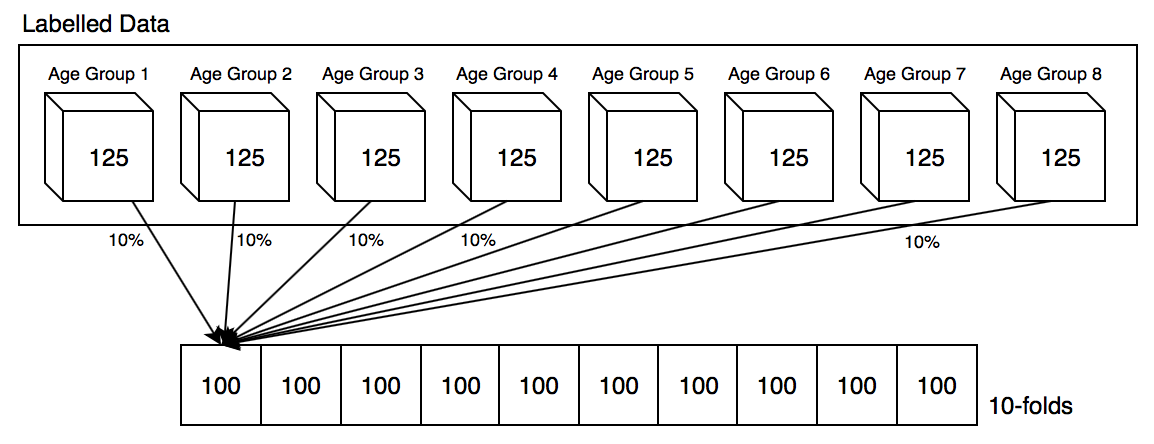
\includegraphics[width=0.88\linewidth]{example-cv.png}
  \caption{Stratified 10-fold cross-validation on 1000 labelled images of 8 different classes}
  \label{fig:example}
\end{figure*}

As concluded by \cite{varma2006bias}, cross-validation is well implemented when everything is taken place within every CV iteration (including preprocessing, feature-selection, learning new algorithm parameter values, etc.), and the least bias can be achieved when using nested CV methods.



\index{class options|)} %TODO


%%
% The back matter contains appendices, bibliographies, indices, glossaries, etc.

\backmatter

\bibliography{terms/crossvalidation_lmd,terms/confusionmatrix_df,terms/activationfunctions_km,terms/convolution_gebs} %TODO
\bibliographystyle{plainnat}

\printindex

\end{document}
